\documentclass[border=10pt]{standalone}
\usepackage{tikz}
\usetikzlibrary{shapes.geometric, arrows}

% Define styles for blocks and arrows
\tikzstyle{startstop} = [rectangle, rounded corners, minimum width=3cm, minimum height=1cm, text centered, draw=black, fill=red!30]
\tikzstyle{process} = [rectangle, minimum width=3cm, minimum height=1cm, text centered, draw=black, fill=blue!30]
\tikzstyle{decision} = [diamond, minimum width=3cm, minimum height=1cm, text centered, draw=black, fill=green!30]
\tikzstyle{arrow} = [thick,->,>=stealth]

\begin{document}
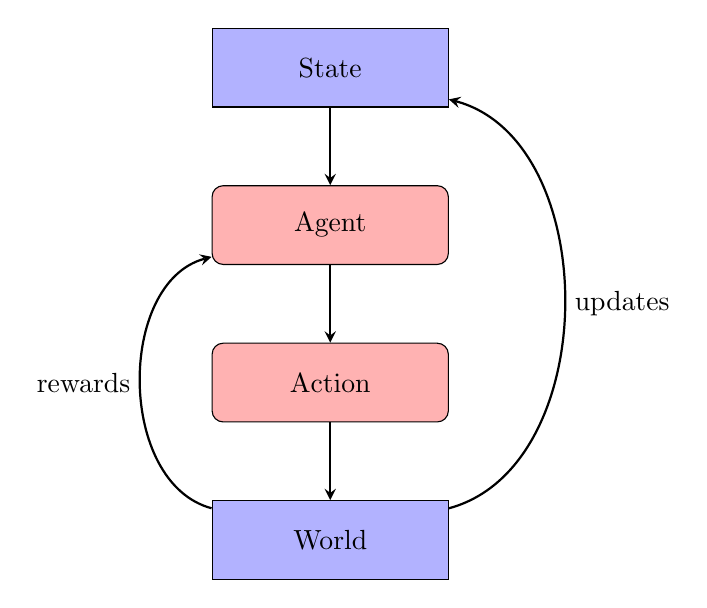
\begin{tikzpicture}[node distance=2cm]
    % Place nodes
    \node (state) [process] {State};
    \node (agent) [startstop, below of=state] {Agent};
    \node (action) [startstop, below of=agent] {Action};
    \node (world) [process, below of=action] {World};
    
    % Connect nodes with arrows
    \draw [arrow] (state) -- (agent);
    \draw [arrow] (agent) -- (action);
    \draw [arrow] (action) -- (world);
    \draw [arrow] (world) to [bend right=75] node[right] {updates} (state);
    \draw [arrow] (world) to [bend left=75] node[left] {rewards} (agent);
\end{tikzpicture}
\end{document}
